\chapter{The 3 components of ML}

Every Machine Learning method, from linear regression to deep neural networks, is built from the same three components:
\begin{itemize}
    \item \textbf{Data}: \emph{what do we learn from?}
    \item \textbf{Model}: \emph{which predictors are we allowed to use?}
    \item \textbf{Loss}: \emph{how do we measure if a predictor is good?}
\end{itemize}

\section{Data}

\textit{``For a lot of problems, we should shift our mindset toward not just improving the code but in a more systematic way of improving the data''.}

Data is a set of \textbf{data points} (also called samples, records or objects). Each data point carries two kinds of information:

\begin{itemize}
    \item \textbf{Features} $x$: \textbf{low-level} properties that are \textbf{easy to measure}. They are mainly numeric and are stacked into a \textbf{feature vector} $x = (x_1, \dots, x_n)$.
    \item \textbf{Label} $y$: the \textbf{high-level quantity of interest}, often \textbf{difficult to determine} (it may require an expert, time or money). The label is a \textbf{design choice}: by choosing what the label is, we are defining the ML problem (the learning task).
\end{itemize}

\emph{Example}: a data point is a network flow. Its features are easy to measure (packet sizes, duration, number of packets, ports). Its label could be the application that generated it (e.g.\ video, VoIP, web), which cannot be read directly from the traffic.

The type of label determines the type of task:
\begin{itemize}
    \item \textbf{Categorical label} $\rightarrow$ \textbf{classification}. With 2 categories it is \emph{binary} classification (e.g.\ normal vs.\ attack); with more than 2 it is \emph{multi-class} classification (e.g.\ video vs.\ VoIP vs.\ web).
    \item \textbf{Numerical label} $\rightarrow$ \textbf{regression} (e.g.\ predicting the throughput of a link).
    \item If a data point has \textbf{more than one label}, the problem is \textbf{multi-label}, and it requires multi-task learning.
\end{itemize}

\begin{figure}[h]
    \centering
    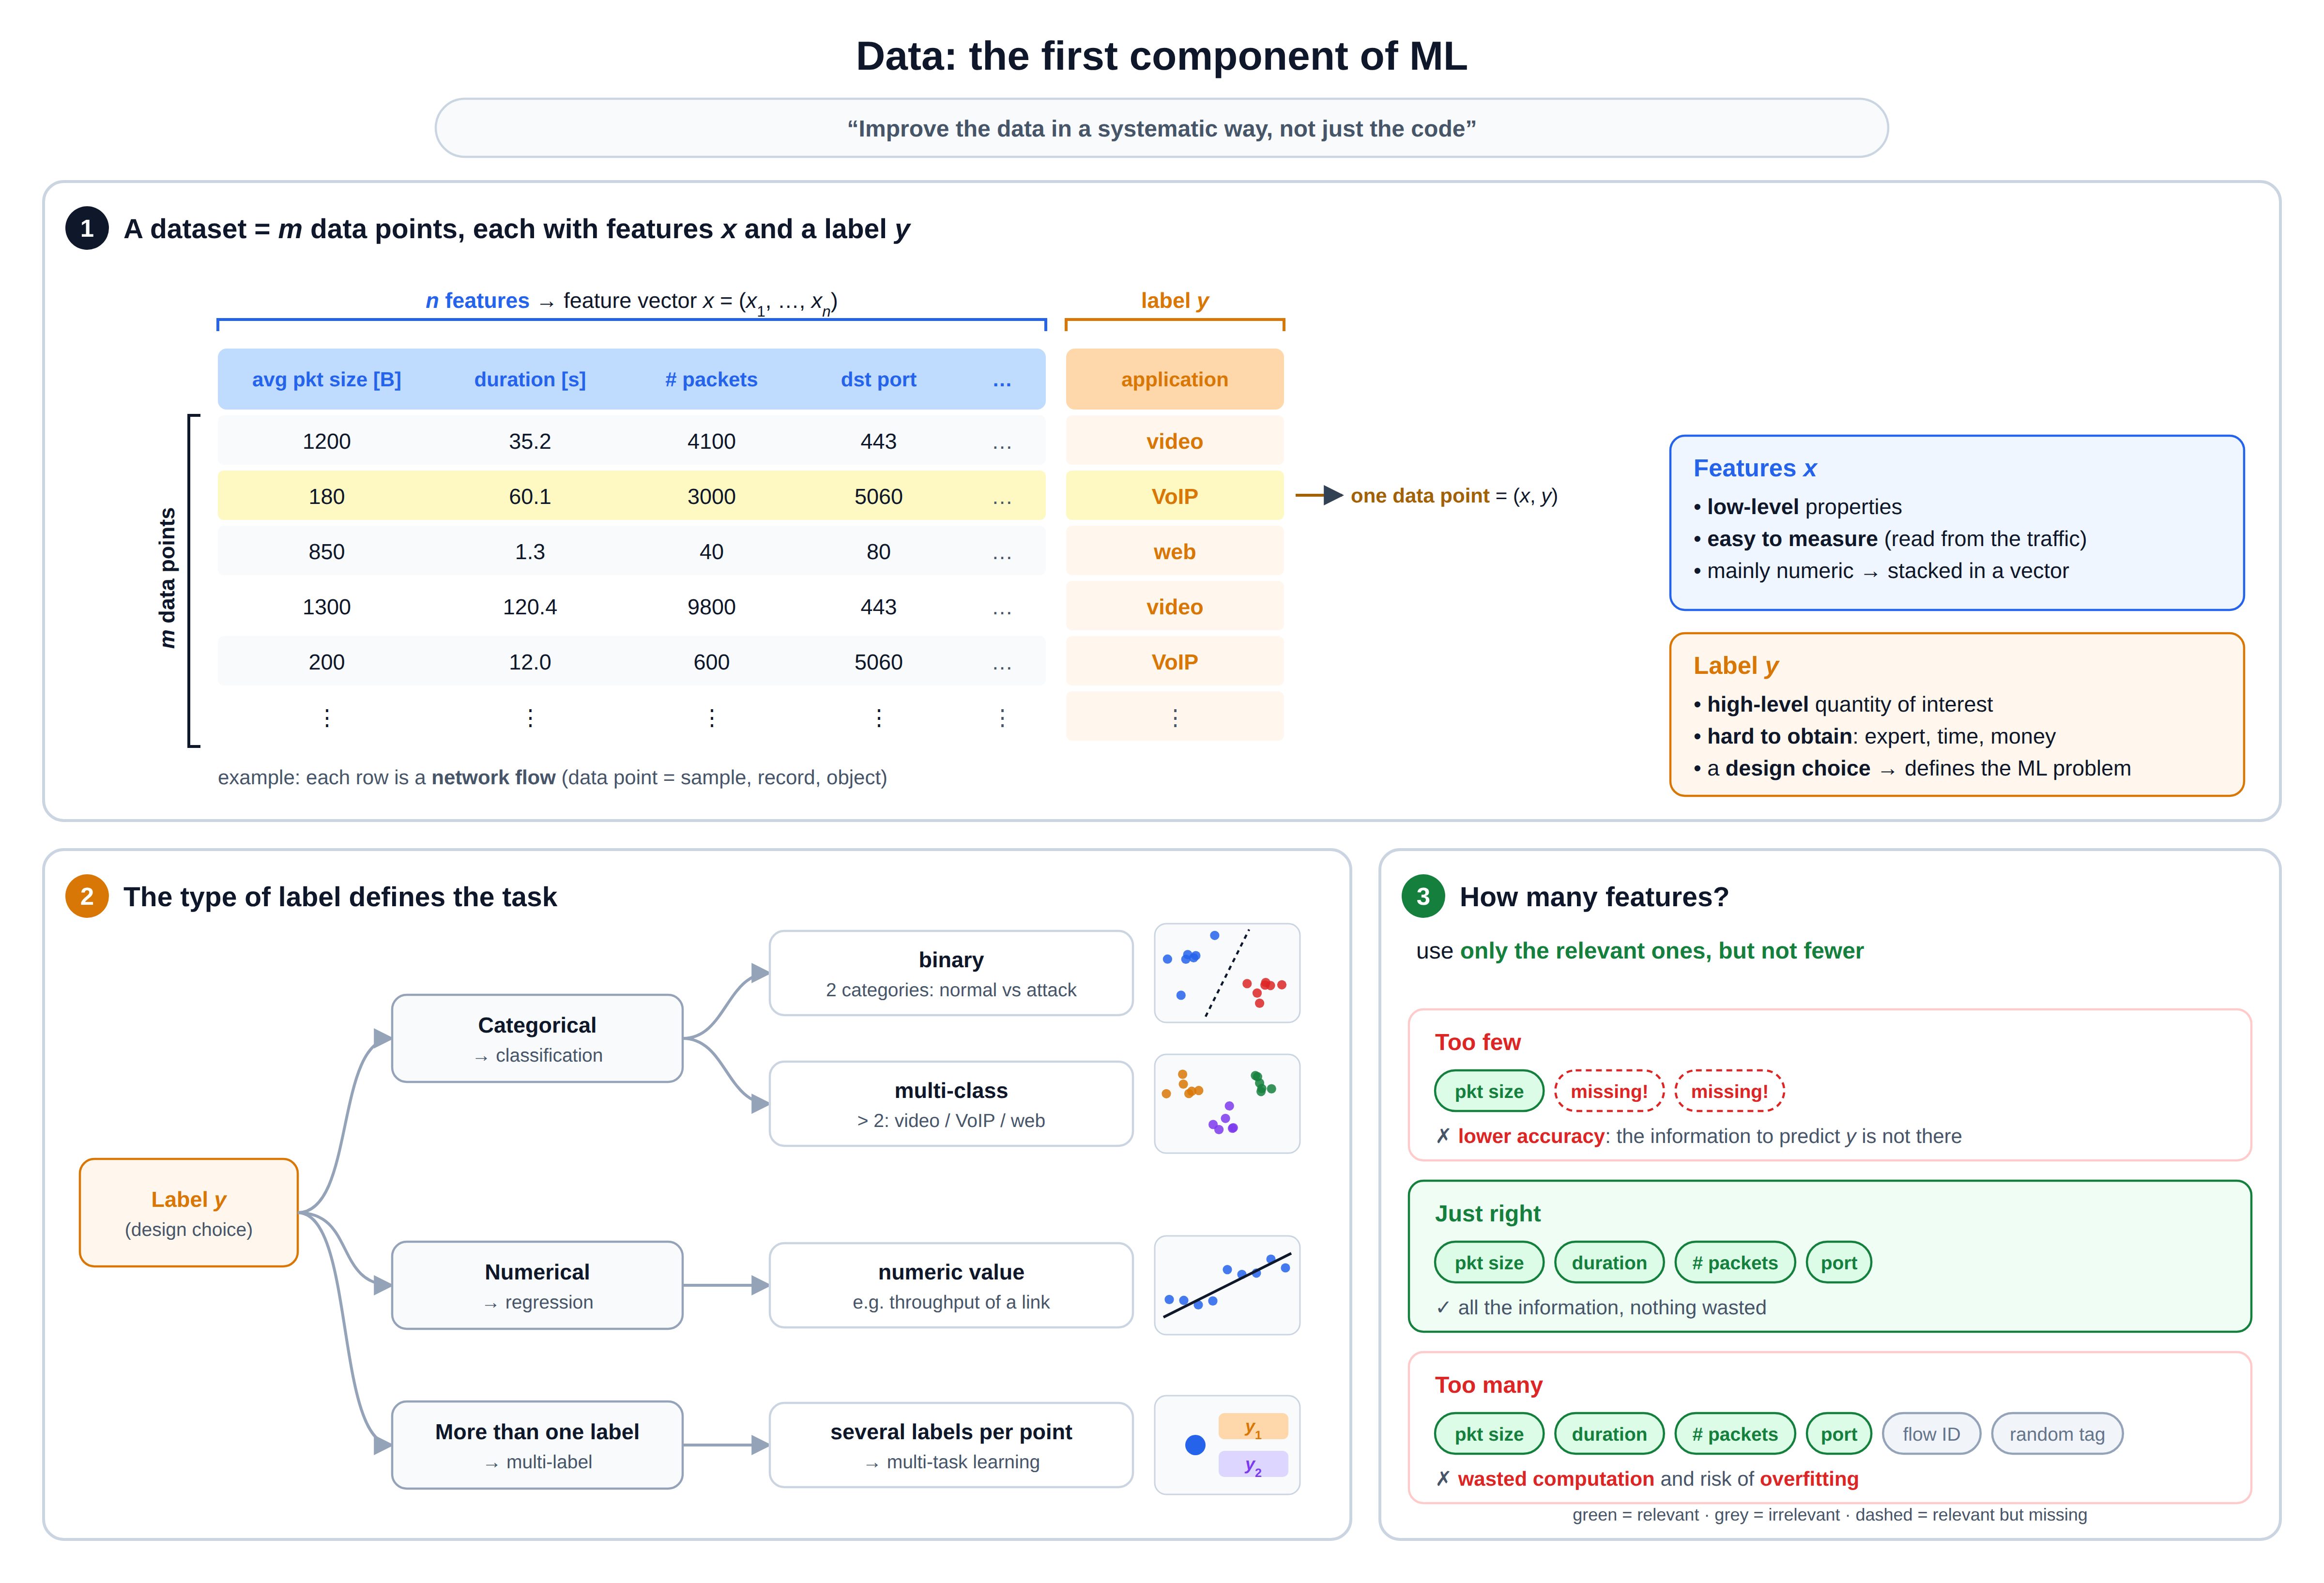
\includegraphics[width=1\textwidth]{images/chapter_5/ml_data.png}
    \caption{Data: data points, features and labels, the type of task, and how many features to use}
\end{figure}

\textbf{Notation}: $m$ is the number of data points, $n$ is the number of features.

\textbf{How many features?} Use \textbf{only the relevant ones, but not fewer}:
\begin{itemize}
    \item missing relevant features hurts \textbf{accuracy}, because the information needed to predict $y$ is not there;
    \item adding irrelevant features \textbf{wastes computation} and may cause \textbf{overfitting}.
\end{itemize}

\section{Model}
Every ML method aims at learning how to \textbf{predict the label $y$ of a data point from its features $x$}. In a nutshell, ML looks for a \textbf{hypothesis} (a predictor map) $h$ such that
\[
    h(x) \approx y
\]
The hypothesis is chosen from a set of candidates $\mathcal{H}$, called the \textbf{hypothesis space}; this set is what we call the \textbf{model}. Different ML methods use different hypothesis spaces: linear maps, polynomials, decision trees, artificial neural networks, and many others. The best hypothesis found during training is then used to find patterns, make predictions or classify new data.

\subsection{Size of the hypothesis space}
The hypothesis space $\mathcal{H}$ is a subset of $\mathcal{Y}^{\mathcal{X}}$, the set of \emph{all} possible maps from the feature space $\mathcal{X}$ to the label space $\mathcal{Y}$. Choosing $\mathcal{H}$ means choosing how large this subset is, and it must be:

\begin{itemize}
    \item \textbf{Large enough} to contain at least one good hypothesis. If $\mathcal{H}$ only contains straight lines but the true relation is curved, no $h$ will ever fit well.
    \item \textbf{Small enough}:
    \begin{itemize}
        \item to fit the \textbf{computational resources} available for learning (fitting) and training;
        \item to avoid \textbf{overfitting}: an analysis that corresponds too closely or exactly to a particular set of data, and may therefore fail to fit additional data. A very large $\mathcal{H}$ can ``memorize'' the training data instead of learning the general pattern.
    \end{itemize}
\end{itemize}

\begin{figure}[h]
    \centering
    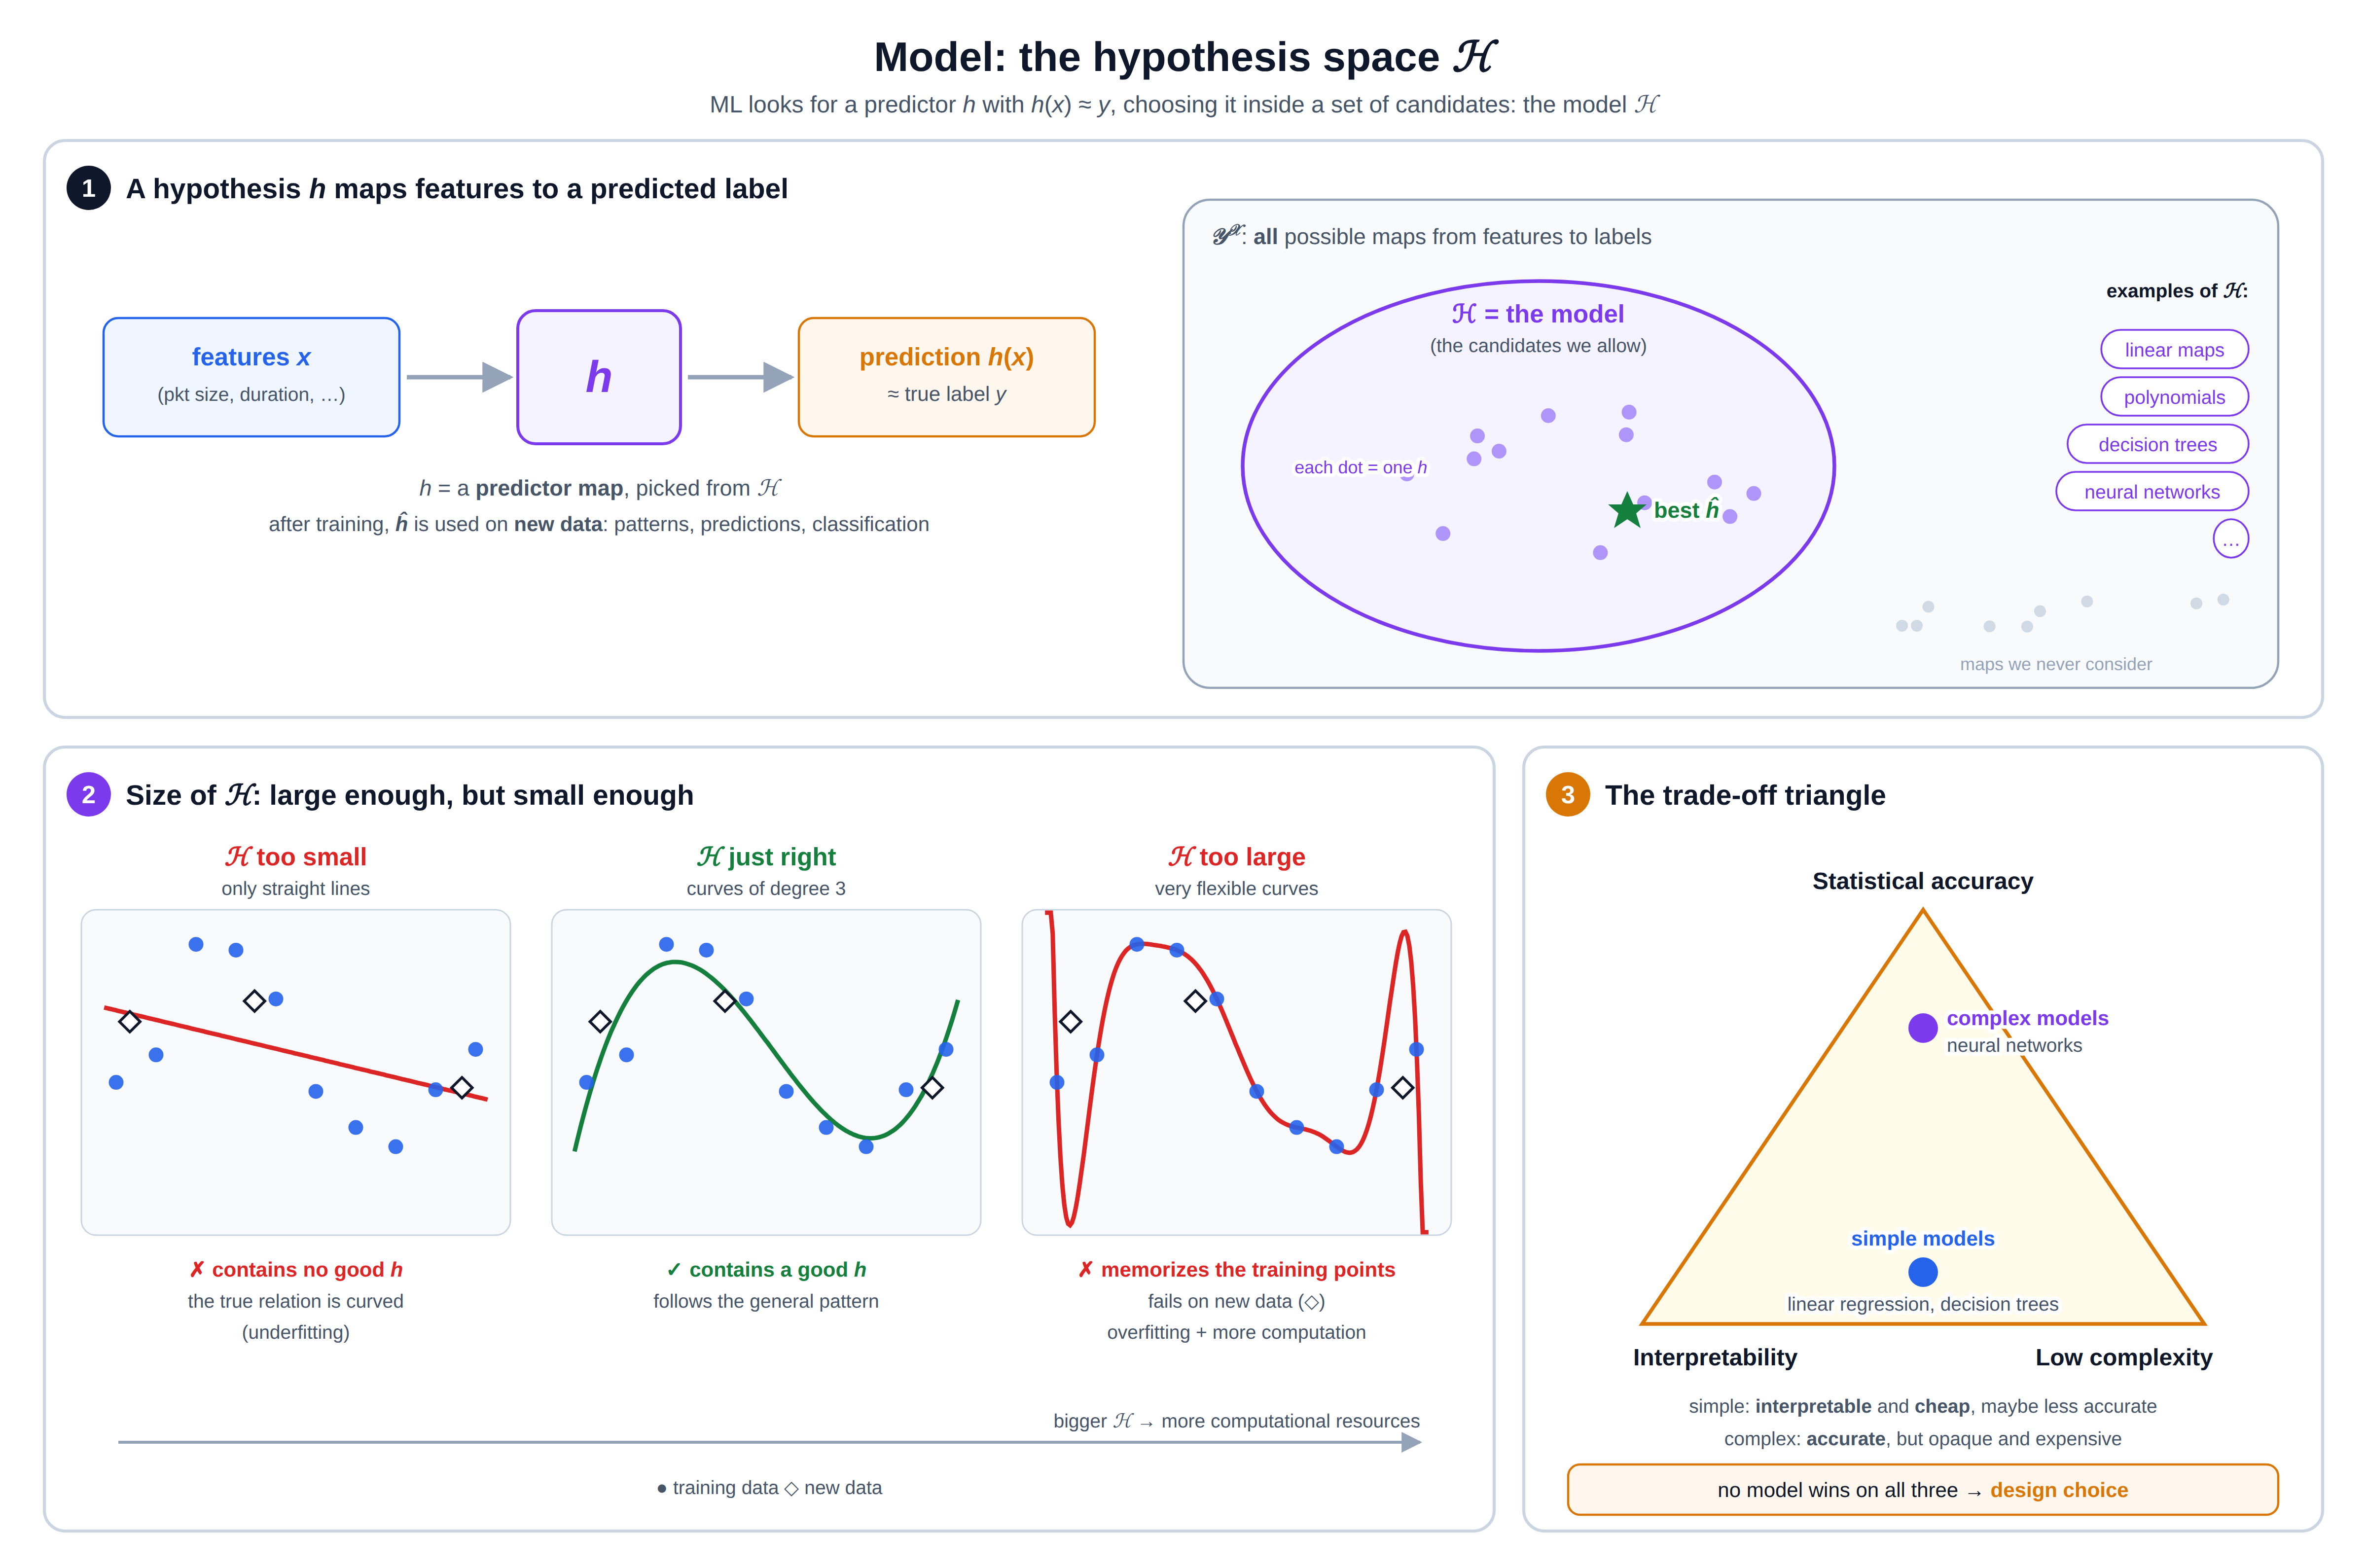
\includegraphics[width=1\textwidth]{images/chapter_5/ml_model.png}
    \caption{Model: the hypothesis space, its size and the trade-off triangle}
\end{figure}

When choosing $\mathcal{H}$ we must balance three competing aspects:
\begin{itemize}
    \item \textbf{Interpretability}: how easily we can understand and explain how the model makes predictions.
    \item \textbf{Statistical accuracy}: how accurate the predictions are.
    \item \textbf{Computational complexity}: the resources needed to train and deploy the model.
\end{itemize}

\textbf{Simple models} (linear regression, decision trees) are interpretable and computationally cheap, but may not reach high accuracy. \textbf{Complex models} (neural networks) can reach high accuracy, but they are harder to interpret and more expensive. There is no universal best choice: finding the right balance in this triangle is a \textbf{design choice}.

\section{Loss}

To decide which hypothesis $h \in \mathcal{H}$ to pick, we need a way to tell good predictors from bad ones. A \textbf{loss function} $L((x,y),h)$ is a quantitative measure of the \textbf{prediction error} we make when we use $h(x)$ to predict the true label $y$ of a data point: the smaller the loss, the better the prediction. Common examples are:
\begin{itemize}
    \item \textbf{Squared error loss}: $L = (y - h(x))^2$, which penalizes large errors heavily;
    \item \textbf{Absolute error loss}: $L = |y - h(x)|$, which is more robust to outliers.
\end{itemize}

\begin{figure}[h]
    \centering
    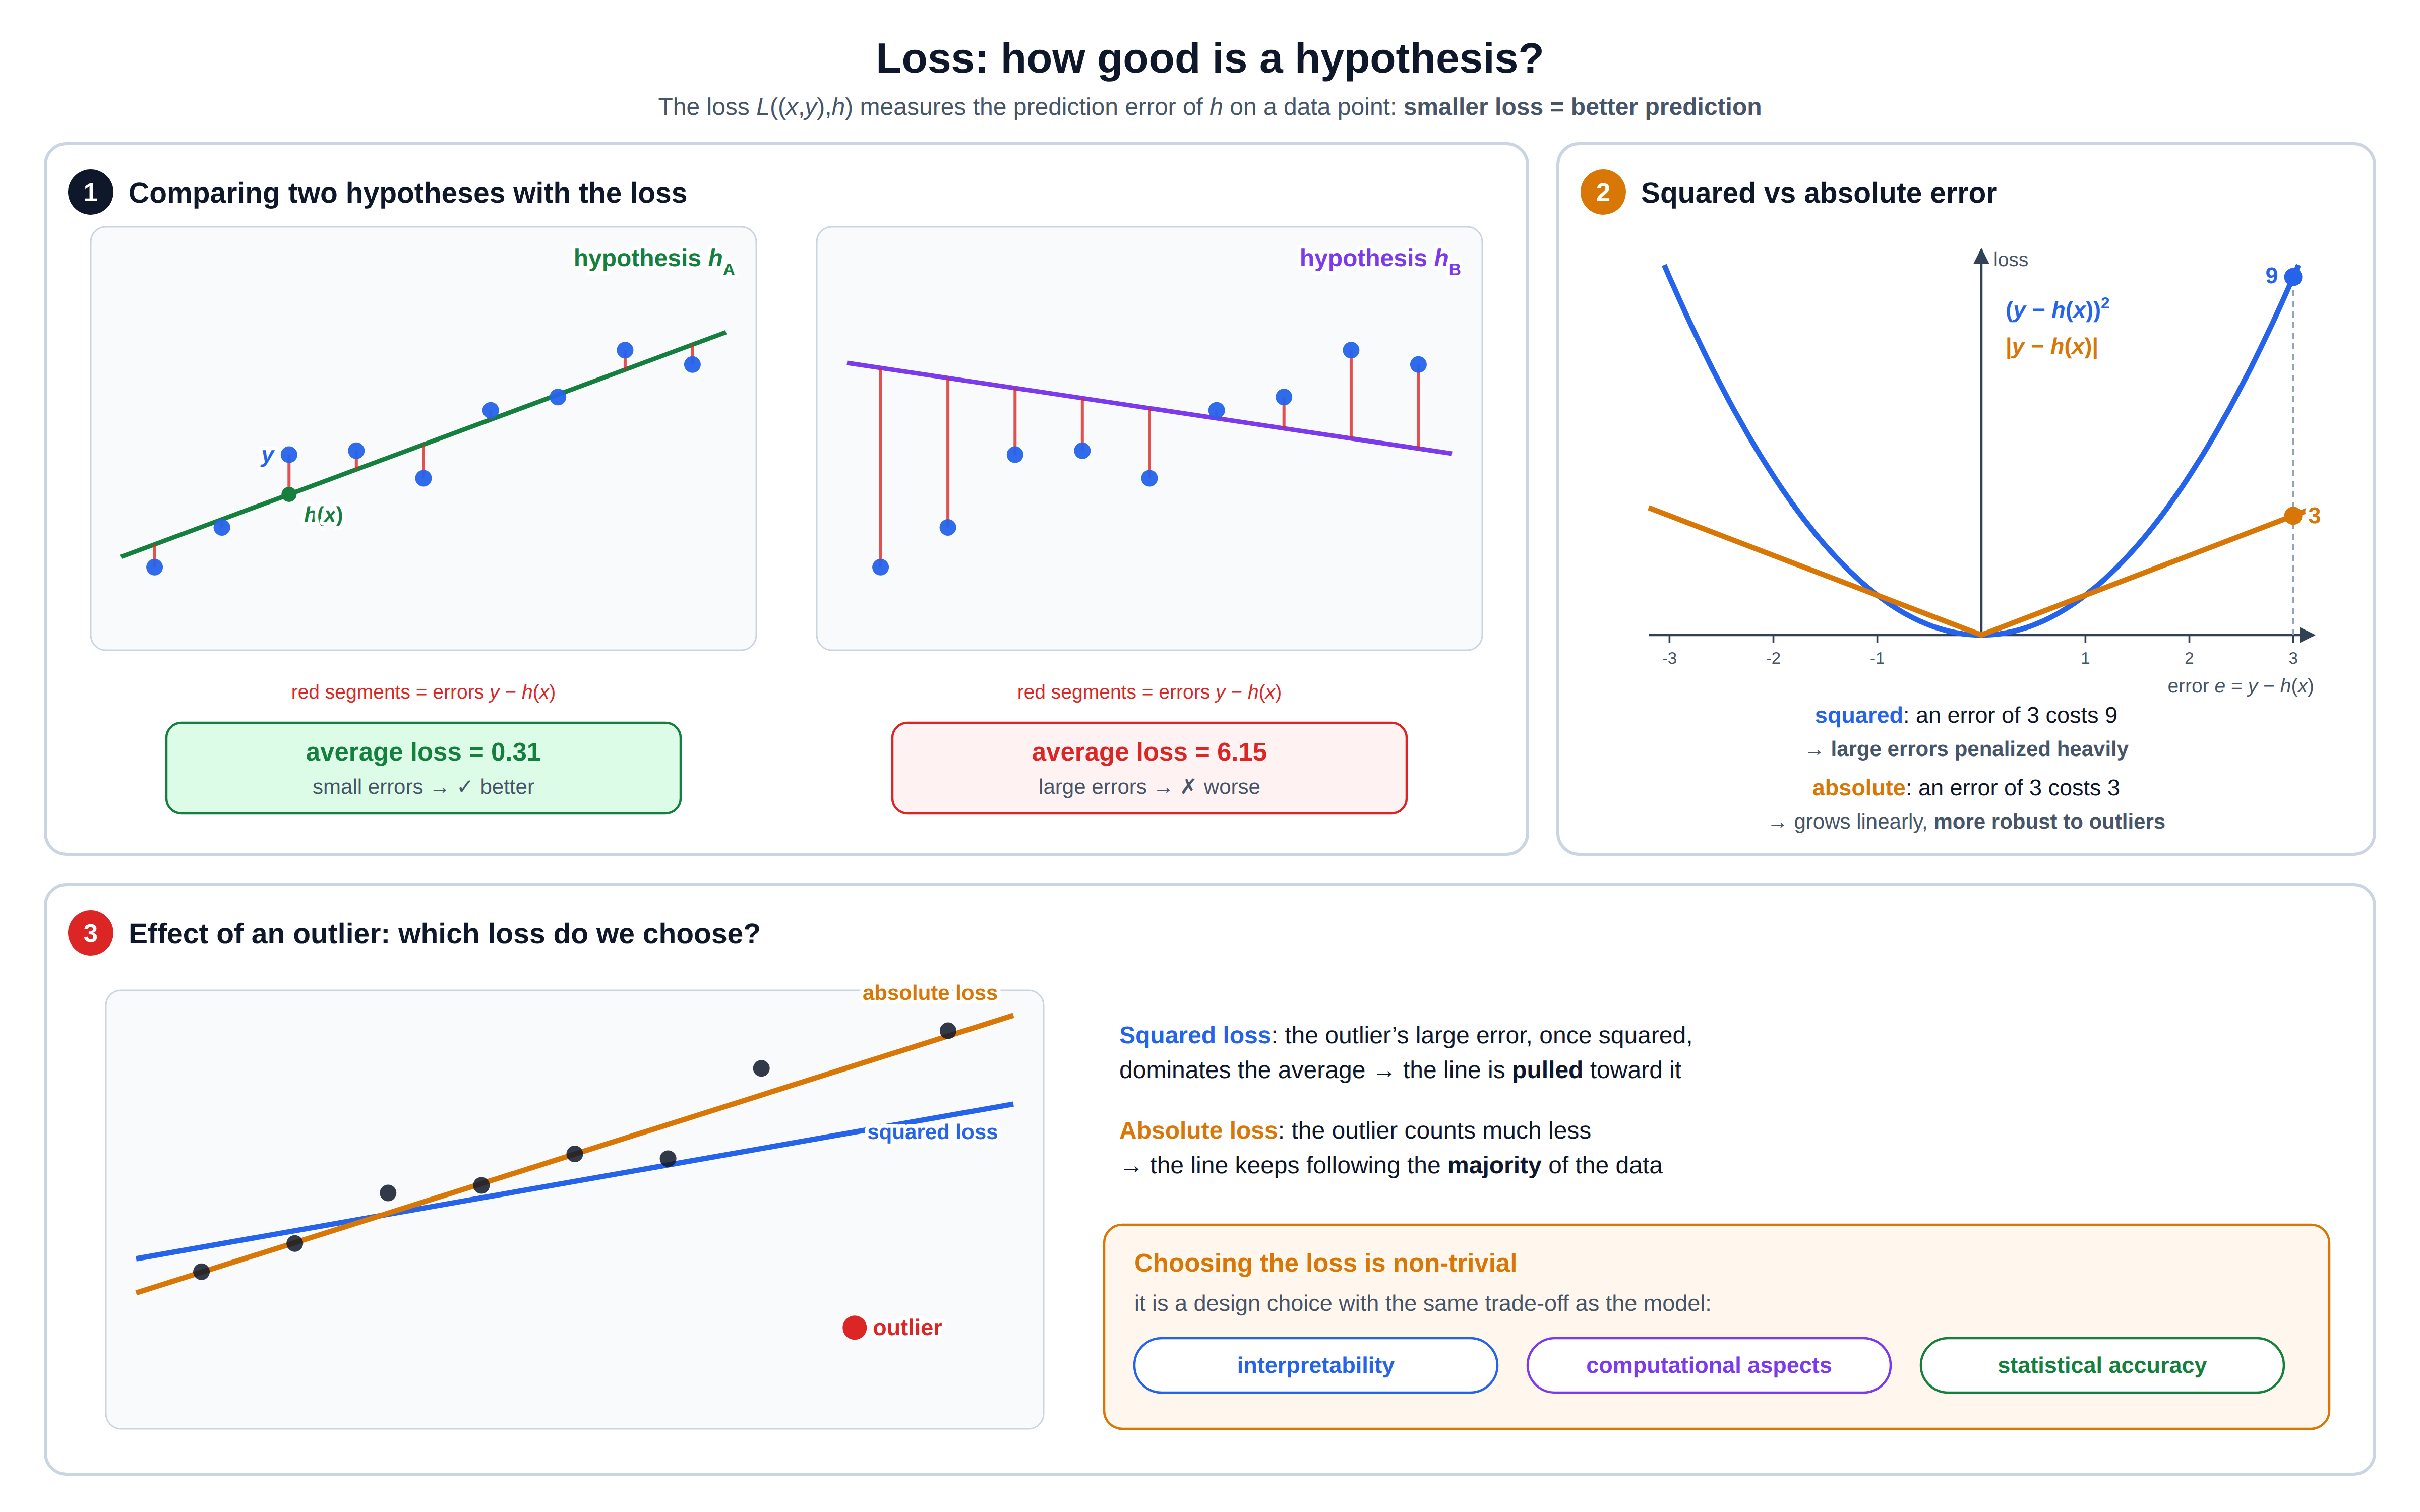
\includegraphics[width=1\textwidth]{images/chapter_5/ml_loss.png}
    \caption{Loss: comparing hypotheses, squared vs absolute error, effect of an outlier}
\end{figure}

Choosing a suitable loss is often non-trivial. Like the model, it involves the trade-off between interpretability, computational aspects and statistical accuracy.

\section{Putting the 3 components together}

Learning means using the \textbf{data} to pick, from the \textbf{model} $\mathcal{H}$, the hypothesis with the smallest \textbf{loss}, on average over the $m$ data points:
\[
    \hat{h} = \arg\min_{h \in \mathcal{H}} \; \frac{1}{m} \sum_{i=1}^{m} L\big((x^{(i)}, y^{(i)}),\, h\big)
\]
The chosen $\hat{h}$ is then used to predict the labels of \textbf{new} data points, for which only the features are known.

Each component also reflects a step of the scientific method:
\begin{itemize}
    \item the \textbf{data} are the \emph{observations};
    \item the \textbf{model} contains the \emph{hypotheses} that try to explain them;
    \item the \textbf{loss} \emph{validates} each hypothesis against the observations, so that we can make accurate predictions and inference on additional observations.
\end{itemize}

\begin{figure}[h]
    \centering
    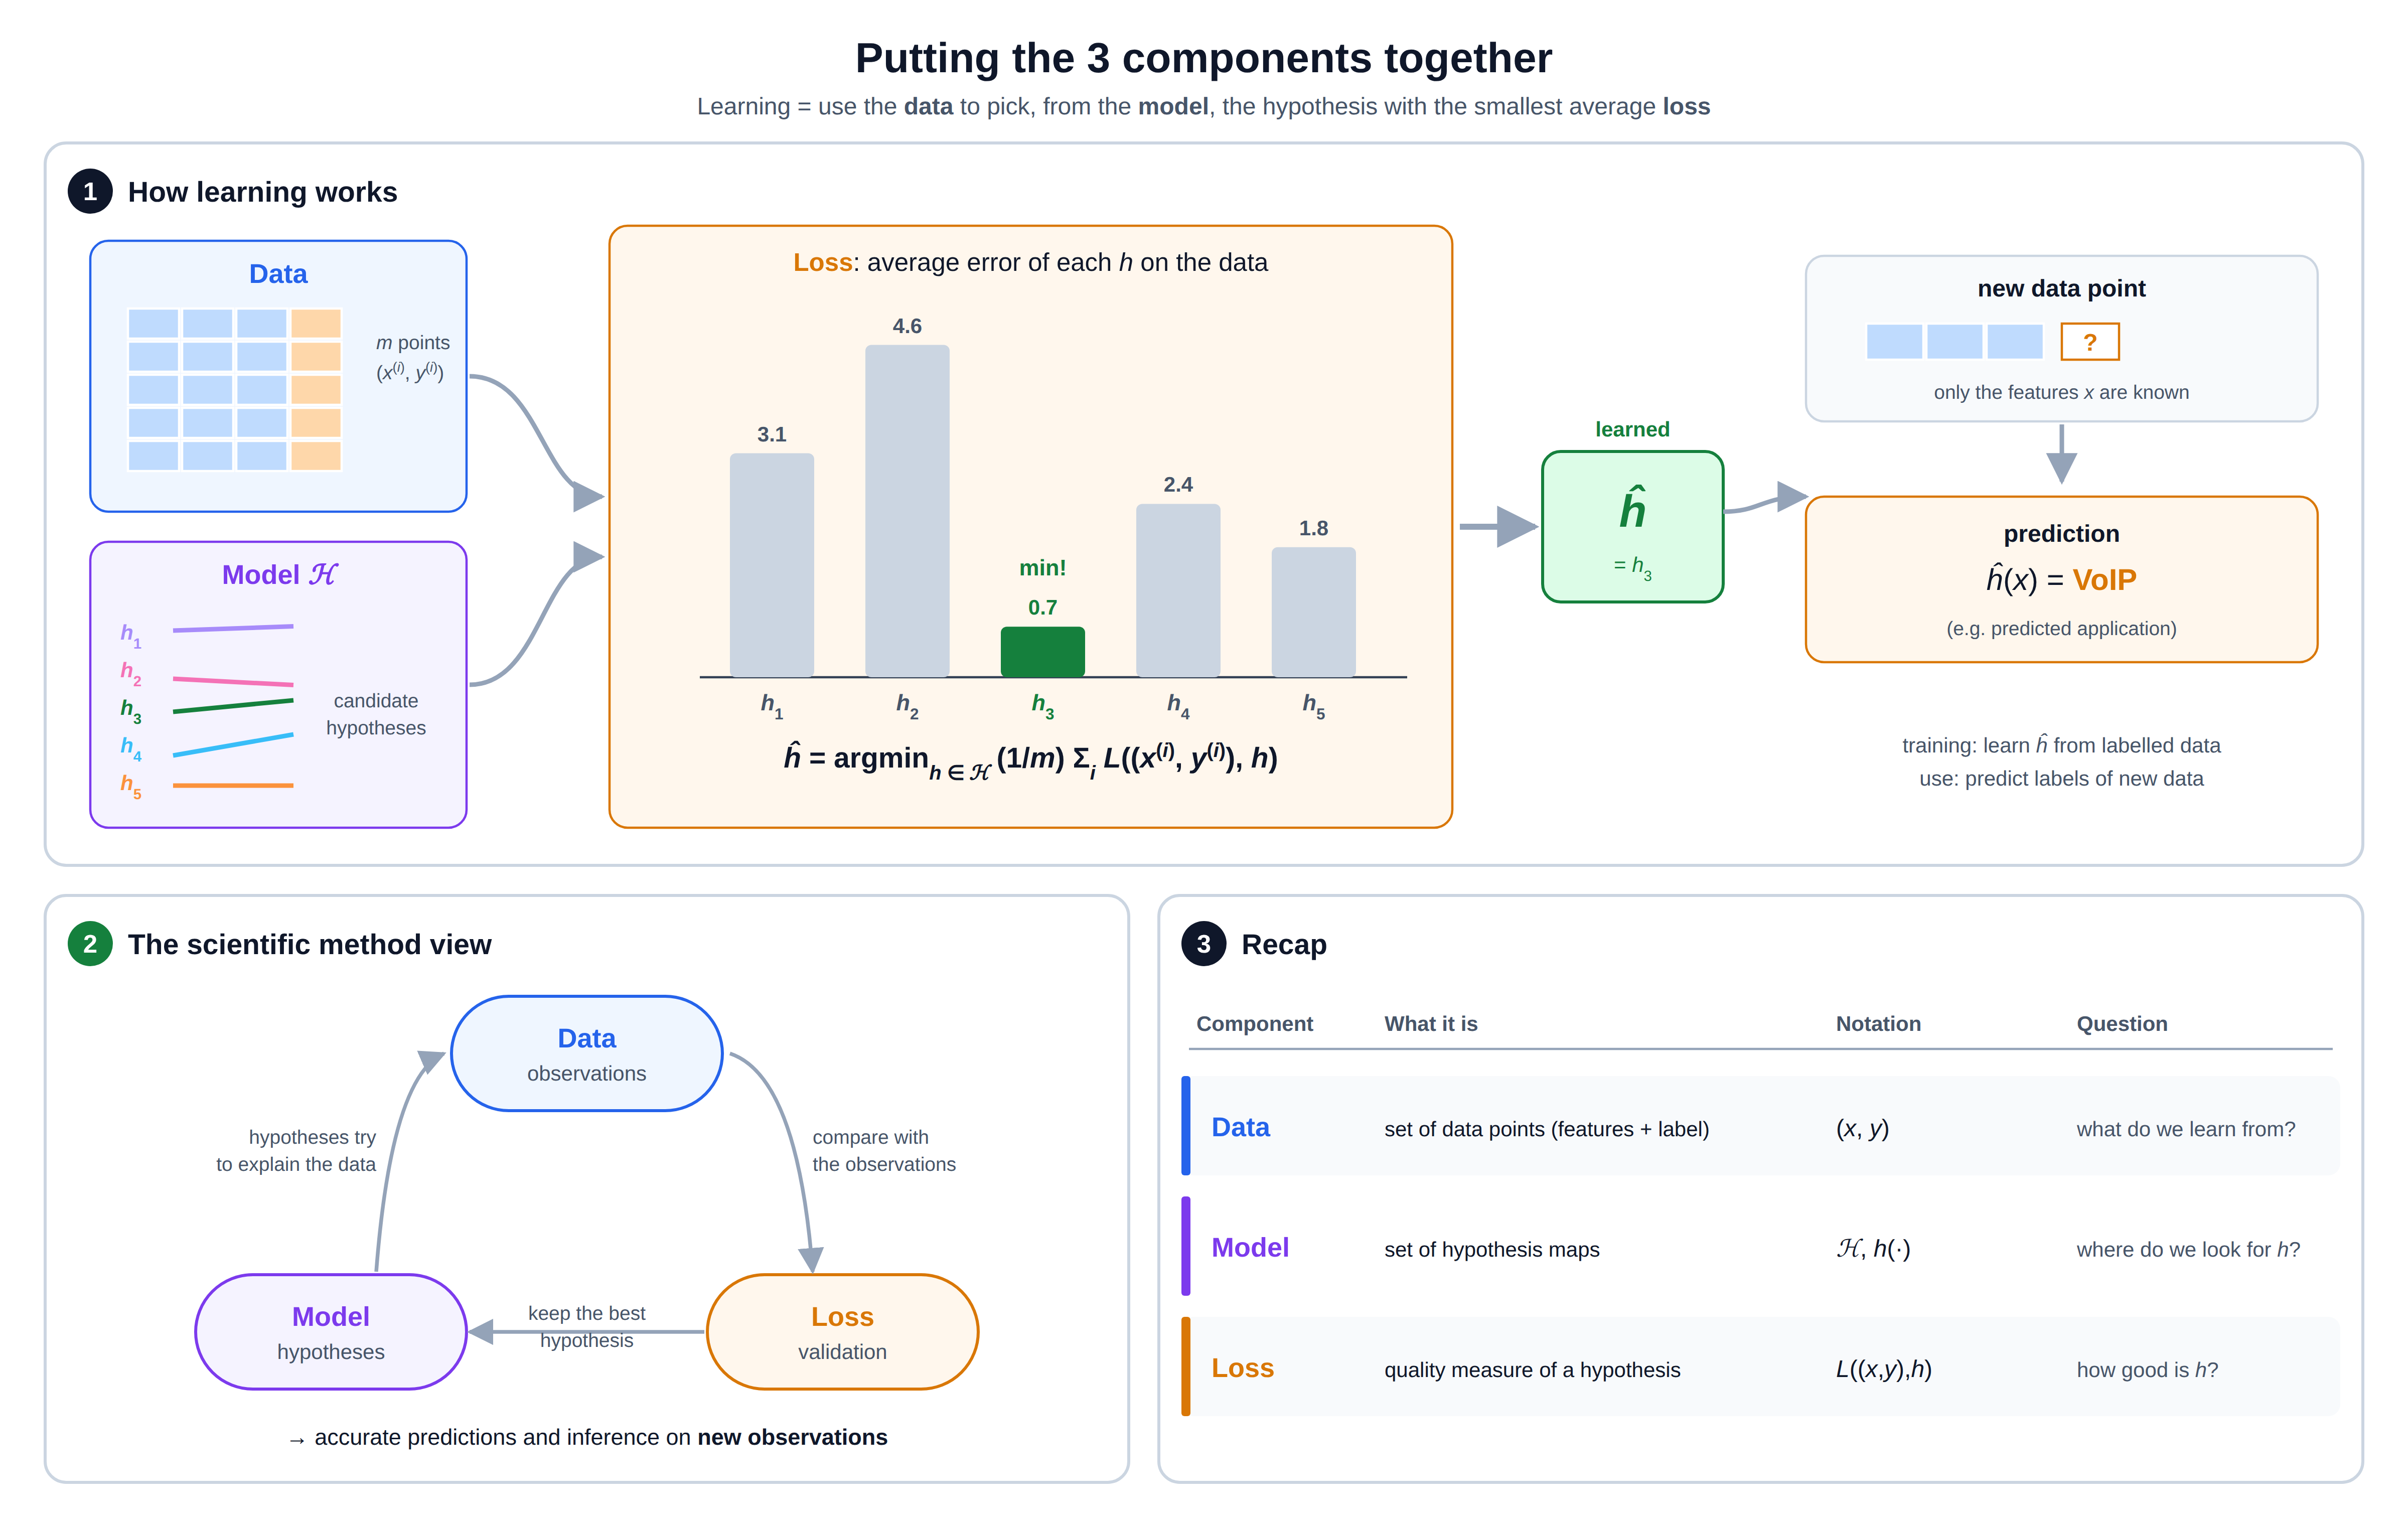
\includegraphics[width=1\textwidth]{images/chapter_5/ml_three_components.png}
    \caption{How data, model and loss work together}
\end{figure}

\begin{center}
    \begin{tabular}{lll}
        \toprule
        \textbf{Component} & \textbf{What it is} & \textbf{Notation} \\
        \midrule
        Data  & set of data points (features + label) & $(x, y)$ \\
        Model & set of hypothesis maps                & $\mathcal{H}$, \ $h(\cdot)$ \\
        Loss  & quality measure of a hypothesis       & $L((x, y), h)$ \\
        \bottomrule
    \end{tabular}
\end{center}


\section{A prova di coglione}

\paragraph*{L'idea di fondo.}
Qualsiasi metodo di Machine Learning, dalla regressione lineare alle reti neurali profonde, nasce dalla combinazione di tre ingredienti: i \textbf{dati}, il \textbf{modello} e la \textbf{loss}. Cambiano i dettagli, ma lo schema è sempre lo stesso. Abbiamo degli esempi da cui imparare, un insieme di possibili ``regole'' tra cui scegliere e un criterio per giudicare quale regola funziona meglio. Capire questi tre elementi significa capire la struttura di ogni algoritmo di ML.

\paragraph*{I dati: da cosa impariamo.}
I dati sono un insieme di $m$ \textbf{data point}, cioè gli esempi. Ognuno porta con sé due tipi di informazione:
\begin{itemize}
    \item le \textbf{feature} $x$: proprietà facili da misurare, raccolte in un vettore di $n$ numeri;
    \item la \textbf{label} $y$: la grandezza che ci interessa davvero, ma che è difficile o costosa da ottenere.
\end{itemize}
In una rete, ad esempio, di un flusso di traffico misuriamo facilmente dimensioni dei pacchetti e durata (le feature), ma vorremmo sapere quale applicazione lo ha generato (la label). Il punto chiave è che \textbf{scegliere la label significa scegliere il problema}:
\begin{itemize}
    \item label a categorie $\rightarrow$ classificazione (binaria o multi-classe);
    \item label numerica $\rightarrow$ regressione;
    \item più label per lo stesso data point $\rightarrow$ problema multi-label.
\end{itemize}
Anche le feature vanno scelte con cura: servono quelle rilevanti, né di più né di meno. Se ne mancano alcune, l'informazione per predire $y$ non c'è. Se ce ne sono troppe inutili, si spreca calcolo e si rischia l'overfitting.

\paragraph*{Il modello: dove cerchiamo la soluzione.}
L'obiettivo del ML è trovare una funzione, l'\textbf{ipotesi} $h$, che a partire dalle feature restituisca una buona stima della label: $h(x) \approx y$. Non la cerchiamo tra tutte le funzioni possibili, ma dentro un insieme scelto da noi, lo \textbf{spazio delle ipotesi} $\mathcal{H}$, che è ciò che chiamiamo \emph{modello}. Scegliere di usare ``solo rette'', ``solo alberi di decisione'' o ``reti neurali'' significa scegliere $\mathcal{H}$.

Quanto deve essere grande questo insieme?
\begin{itemize}
    \item \textbf{Abbastanza grande} da contenere una buona soluzione: se cerco solo tra le rette e il fenomeno è curvo, non la troverò mai.
    \item \textbf{Abbastanza piccolo} da essere gestibile con le risorse di calcolo, e soprattutto da evitare l'\textbf{overfitting}. Un modello troppo ricco può ``imparare a memoria'' i dati di training invece di coglierne lo schema generale, e poi sbaglia sui dati nuovi.
\end{itemize}
Nella scelta entra in gioco un \textbf{triangolo di compromessi} tra interpretabilità, accuratezza e costo computazionale:
\begin{itemize}
    \item i modelli semplici sono comprensibili ed economici, ma a volte poco precisi;
    \item i modelli complessi sono precisi, ma opachi e costosi.
\end{itemize}
Non esiste una scelta giusta in assoluto: è una decisione di progetto.

\paragraph*{La loss: come giudichiamo una soluzione.}
Dentro $\mathcal{H}$ ci sono moltissime ipotesi, e per sceglierne una serve un criterio numerico. La \textbf{loss} $L((x,y),h)$ misura quanto sbaglia l'ipotesi $h$ su un data point, confrontando la predizione $h(x)$ con la vera label $y$: più è bassa, meglio è. L'errore si può misurare in modi diversi:
\begin{itemize}
    \item l'\textbf{errore quadratico} punisce molto gli errori grandi;
    \item l'\textbf{errore assoluto} è più tollerante verso i valori anomali.
\end{itemize}
Anche questa scelta non è banale e risente dello stesso triangolo di compromessi.

\paragraph*{Il meccanismo: come i tre pezzi lavorano insieme.}
Imparare significa usare i \textbf{dati} per scegliere, tra tutte le ipotesi del \textbf{modello}, quella con la \textbf{loss} media più bassa sugli esempi disponibili:
\[
    \hat{h} = \arg\min_{h \in \mathcal{H}} \frac{1}{m}\sum_{i=1}^{m} L\big((x^{(i)},y^{(i)}),h\big)
\]
Una volta trovata, $\hat{h}$ viene usata su data point \textbf{nuovi}, di cui conosciamo solo le feature, per predirne la label.

È lo stesso ragionamento del metodo scientifico:
\begin{itemize}
    \item i dati sono le \emph{osservazioni};
    \item il modello contiene le \emph{ipotesi} che provano a spiegarle;
    \item la loss è la \emph{verifica} che ci dice quale ipotesi regge meglio il confronto con la realtà.
\end{itemize}

\paragraph*{Da ricordare.}
\begin{itemize}
    \item \textbf{Dati}: esempi $(x, y)$. Le feature si misurano facilmente, la label è ciò che vogliamo predire, e la sua scelta definisce il problema.
    \item \textbf{Modello}: l'insieme $\mathcal{H}$ in cui cerchiamo $h$. Né troppo piccolo (non contiene la soluzione) né troppo grande (overfitting, costi).
    \item \textbf{Loss}: il voto numerico che misura l'errore di $h$.
    \item \textbf{Apprendimento}: scegliere in $\mathcal{H}$ l'ipotesi che sui dati ha la loss media minima.
\end{itemize}